% \pdfminorversion=4
\documentclass{beamer}
\usepackage[utf8]{inputenc}
\usepackage{indentfirst}
\usepackage{enumitem}
\usepackage{datetime2}
\usepackage{acronym}
% options (https://tex.stackexchange.com/questions/25520/how-can-i-use-the-latex-acronym-package-and-optionally-create-an-acronym-list-i):
% printonlyused: Only list used acronyms
% withpage: In printonlyused-mode show the page number where each acronym was first used.
% nolist: The option nolist stands for “don’t write the list of acronyms”.
% dua: The option dua stands for “don’t use acronyms”. It leads to a redefinition of \ac and \acp, making the full name appear all the time and suppressing all acronyms but the explicity requested by \acf or \acfp.

\makeatletter
\AtBeginDocument{%
  \renewcommand*{\AC@hyperlink}[2]{%
    \begingroup
      \hypersetup{hidelinks}%
      \hyperlink{#1}{#2}%
    \endgroup
  }%
}
\makeatother

\usepackage{algorithm}
\usepackage{algpseudocode}

\usepackage{textcomp}
\usepackage[T1]{fontenc}
\usepackage{multirow,bigdelim}
\usepackage{float}
\usepackage[caption = false]{subfig}
\usepackage{longtable}
\usepackage{listings}
\usepackage{mathtools}
\DeclareMathOperator{\tr}{Tr}
\usepackage{commath}
\usepackage{slashed}
\usepackage{bbold}
\usepackage{xcolor}
\usepackage{physics}
\newcommand{\lambdabar}{{\mkern0.75mu\mathchar '26\mkern -9.75mu\lambda}}
\usepackage[right=4cm,left=2cm,top=3cm,bottom=3.0cm, marginparwidth=2.7cm, marginparsep=3mm]{geometry}
\usepackage{mdframed}


\usepackage{amsmath}
\usepackage{amsfonts}
\usepackage{amssymb}

\numberwithin{equation}{section}
\usepackage{graphicx}

\usepackage[colorinlistoftodos]{todonotes}
\PassOptionsToPackage{hyphens}{url}
\usepackage[colorlinks=true, allcolors=blue]{hyperref}
\hypersetup{breaklinks=true}

% \urlstyle{same}
\usepackage{siunitx}
\sisetup{separate-uncertainty=true}
% \DeclareSIUnit\parsec{pc}
\usepackage{cancel}
\usepackage{mathrsfs}
\usepackage{marginnote}
\renewcommand*{\marginnotevadjust}{-0.3cm}
\renewcommand*{\marginfont}{\scriptsize}
% \usepackage{fancybox}

\usepackage{footnotebackref}

\usepackage[sc]{mathpazo}
\linespread{1.05}         % Palladio needs more leading (space between lines)
\usepackage[T1]{fontenc}

\newcommand\mybox[1]{%
  \fbox{\begin{minipage}{0.9\textwidth}#1\end{minipage}}}

\newcommand{\const}{\mathrm{const}}

\usepackage[section]{placeins}

\usepackage{tikz}
\usetikzlibrary{shapes,arrows,shadows}


\newcommand{\boxalign}[2][0.986\textwidth]{
  \par\noindent\tikzstyle{mybox} = [draw=black,inner sep=6pt]
  \begin{center}\begin{tikzpicture}
   \node [mybox] (box){%
    \begin{minipage}{#1}{\vspace{-5mm}#2}\end{minipage}
   };
\end{tikzpicture}\end{center}}


\pagestyle{plain}

\author{Jacopo Tissino}

\allowdisplaybreaks
\usetheme{Rochester}
% \usepackage[scaled]{helvet} % ss

\usepackage[
backend=biber,
style=authoryear,
sorting=nyt,
urldate=iso8601,
url=false,
isbn=false,
doi=false
]{biblatex}

\title{Machine Learning for Gravitational Waveforms from Binary Neutron Star mergers}
\author{Jacopo Tissino \\ Advisors: Dr.\ Sebastiano Bernuzzi, Dr.\ Michela Mapelli}
\date{2021-10-21}

\addbibresource{../notes/Masters_thesis.bib}

\begin{document}

\frame{\titlepage}

\section{Main presentation}

\begin{frame}
    \frametitle{GW170817: the first BNS merger detection}
    \begin{columns}
        
    \begin{column}{0.5\textwidth}
    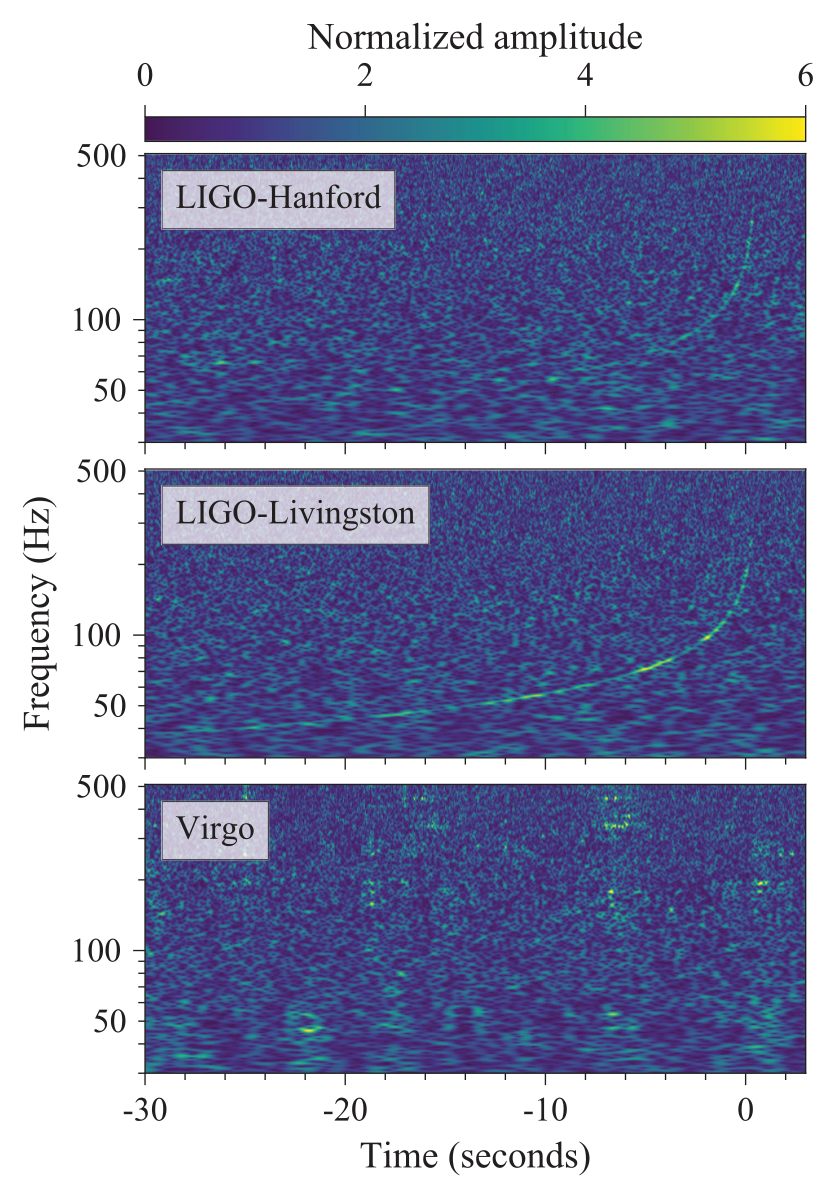
\includegraphics[width=\textwidth]{figures/836px-GW170817_spectrograms.svg.png}
    \end{column}

    \begin{column}{0.5\textwidth}
    Time-frequency representation of the chirping waveform
    (\cite[]{abbottGW170817ObservationGravitational2017}).

    % BNS waveforms are much longer than BBH ones: they only depend on \(t/M \) (or \(fM\)), where \(M = m_1 + m_2 \) is the total mass.
    \end{column}
    \end{columns}
\end{frame}

\begin{frame}
    \frametitle{BBH merger waveform}
    \begin{figure}[ht]
    \centering
    \includegraphics[width=\textwidth]{figures/bbh}
    \label{fig:bbh}
    \end{figure}
\end{frame}

\begin{frame}
    \frametitle{BNS merger waveform}
    \begin{figure}[ht]
    \centering
    \includegraphics[width=\textwidth]{figures/bns}
    \label{fig:bns}
    \end{figure}
\end{frame}

\begin{frame}
    \frametitle{The basics of GW data analysis}
    The signal is modelled as \(s(t) = h_\theta (t) + n(t)\), where: 
    \begin{itemize}
        \item the noise \(n(t)\) is taken to be stationary, with zero mean, and Gaussian with power spectral density \(S_n(f)\);
        \item the signal \(h_\theta (t)\) from a binary neutron star merger depends on: 
        \begin{itemize}
            \item intrinsic parameters: mass ratio \(q = m_1 / m_2 \), spins \(\vec{\chi}_{1}\) and \(\vec{\chi}_2\), tidal polarizabilities \(\Lambda_1\) and \(\Lambda_2 \);
            \item extrinsic parameters: total mass \(M = m_1 + m_2 \), luminosity distance \(D_L\), inclination \(\iota \)\dots
        \end{itemize}
    \end{itemize}
\end{frame}

\begin{frame}
    \frametitle{The Wiener distance}
    
    The likelihood used in parameter estimation reads (\cite[]{maggioreGravitationalWavesVolume2007}): 
    %
    \begin{align}
    \Lambda (s | \theta ) \propto \exp( (h_\theta | s) - \frac{1}{2} (h_\theta | h_\theta ))
    \,,
    \end{align}
    %
    where \((a | b)\) is the Wiener product: 
    %
    \begin{align}
    (a | b) = 4 \Re \int_{0}^{\infty } \frac{\widetilde{a}^{*}(f) \widetilde{b} (f)}{S_n (f)} \dd{f}
    \,.
    \end{align}
\end{frame}

\begin{frame}
    \frametitle{Models and accuracy}
    The main strategies for the generation of theoretical waveforms are: 
    \begin{itemize}
        \item numerical relativity;
        \item effective one body;
        \item post-Newtonian.
    \end{itemize}
    
    Their accuracy is computed according to the \textbf{mismatch}
    %
    \begin{align}
        \mathcal{F}[h_1, h_2 ] = 1 - \max_{t_0 , \phi_0 } \underbrace{\frac{(h_1 | h_2 (t_0, \phi_0 ))}{\sqrt{(h_1 | h_1 ) (h_2 | h_2 )}}}_{\cos \theta }
        \,.
    \end{align}
\end{frame}

\begin{frame}
    \frametitle{Amplitudes}
    \begin{figure}[ht]
    \centering
    \includegraphics[width=\textwidth]{figures/native_amplitudes}
    \label{fig:native_amplitudes}
    \end{figure}
\end{frame}

\begin{frame}
    \frametitle{Phases}
    \begin{figure}[ht]
    \centering
    \includegraphics[width=\textwidth]{figures/native_phases}
    \label{fig:native_phases}
    \end{figure}
\end{frame}

% \begin{frame}
%     \frametitle{MLGW\_BNS structure: training dataset generation}
%     \begin{itemize}
%     \item Greedy adaptive downsampling fit;
%     \item EOB waveform generation and downsampling;
%     \item residuals from PN waveforms: \(\Delta A = \log (A _{\text{EOB}}/ A _{\text{PN}})\) and \(\Delta \Phi = \Phi _{\text{EOB}} - \Phi _{\text{PN}}\);
%     \item PCA on the combined, downsampled, rescaled residuals;
%     \item a NN learns the map \(\theta \to PC_i \lambda_i^{\alpha}\);
%     \item the hyperparameters of the NN and \(\alpha \) are optimized case-by-case.
%     \end{itemize}
% \end{frame}

\begin{frame}
    \frametitle{\texttt{mlgw\_bns} structure}
    \vspace*{-.3cm}
    \begin{figure}[ht]
    \centering
    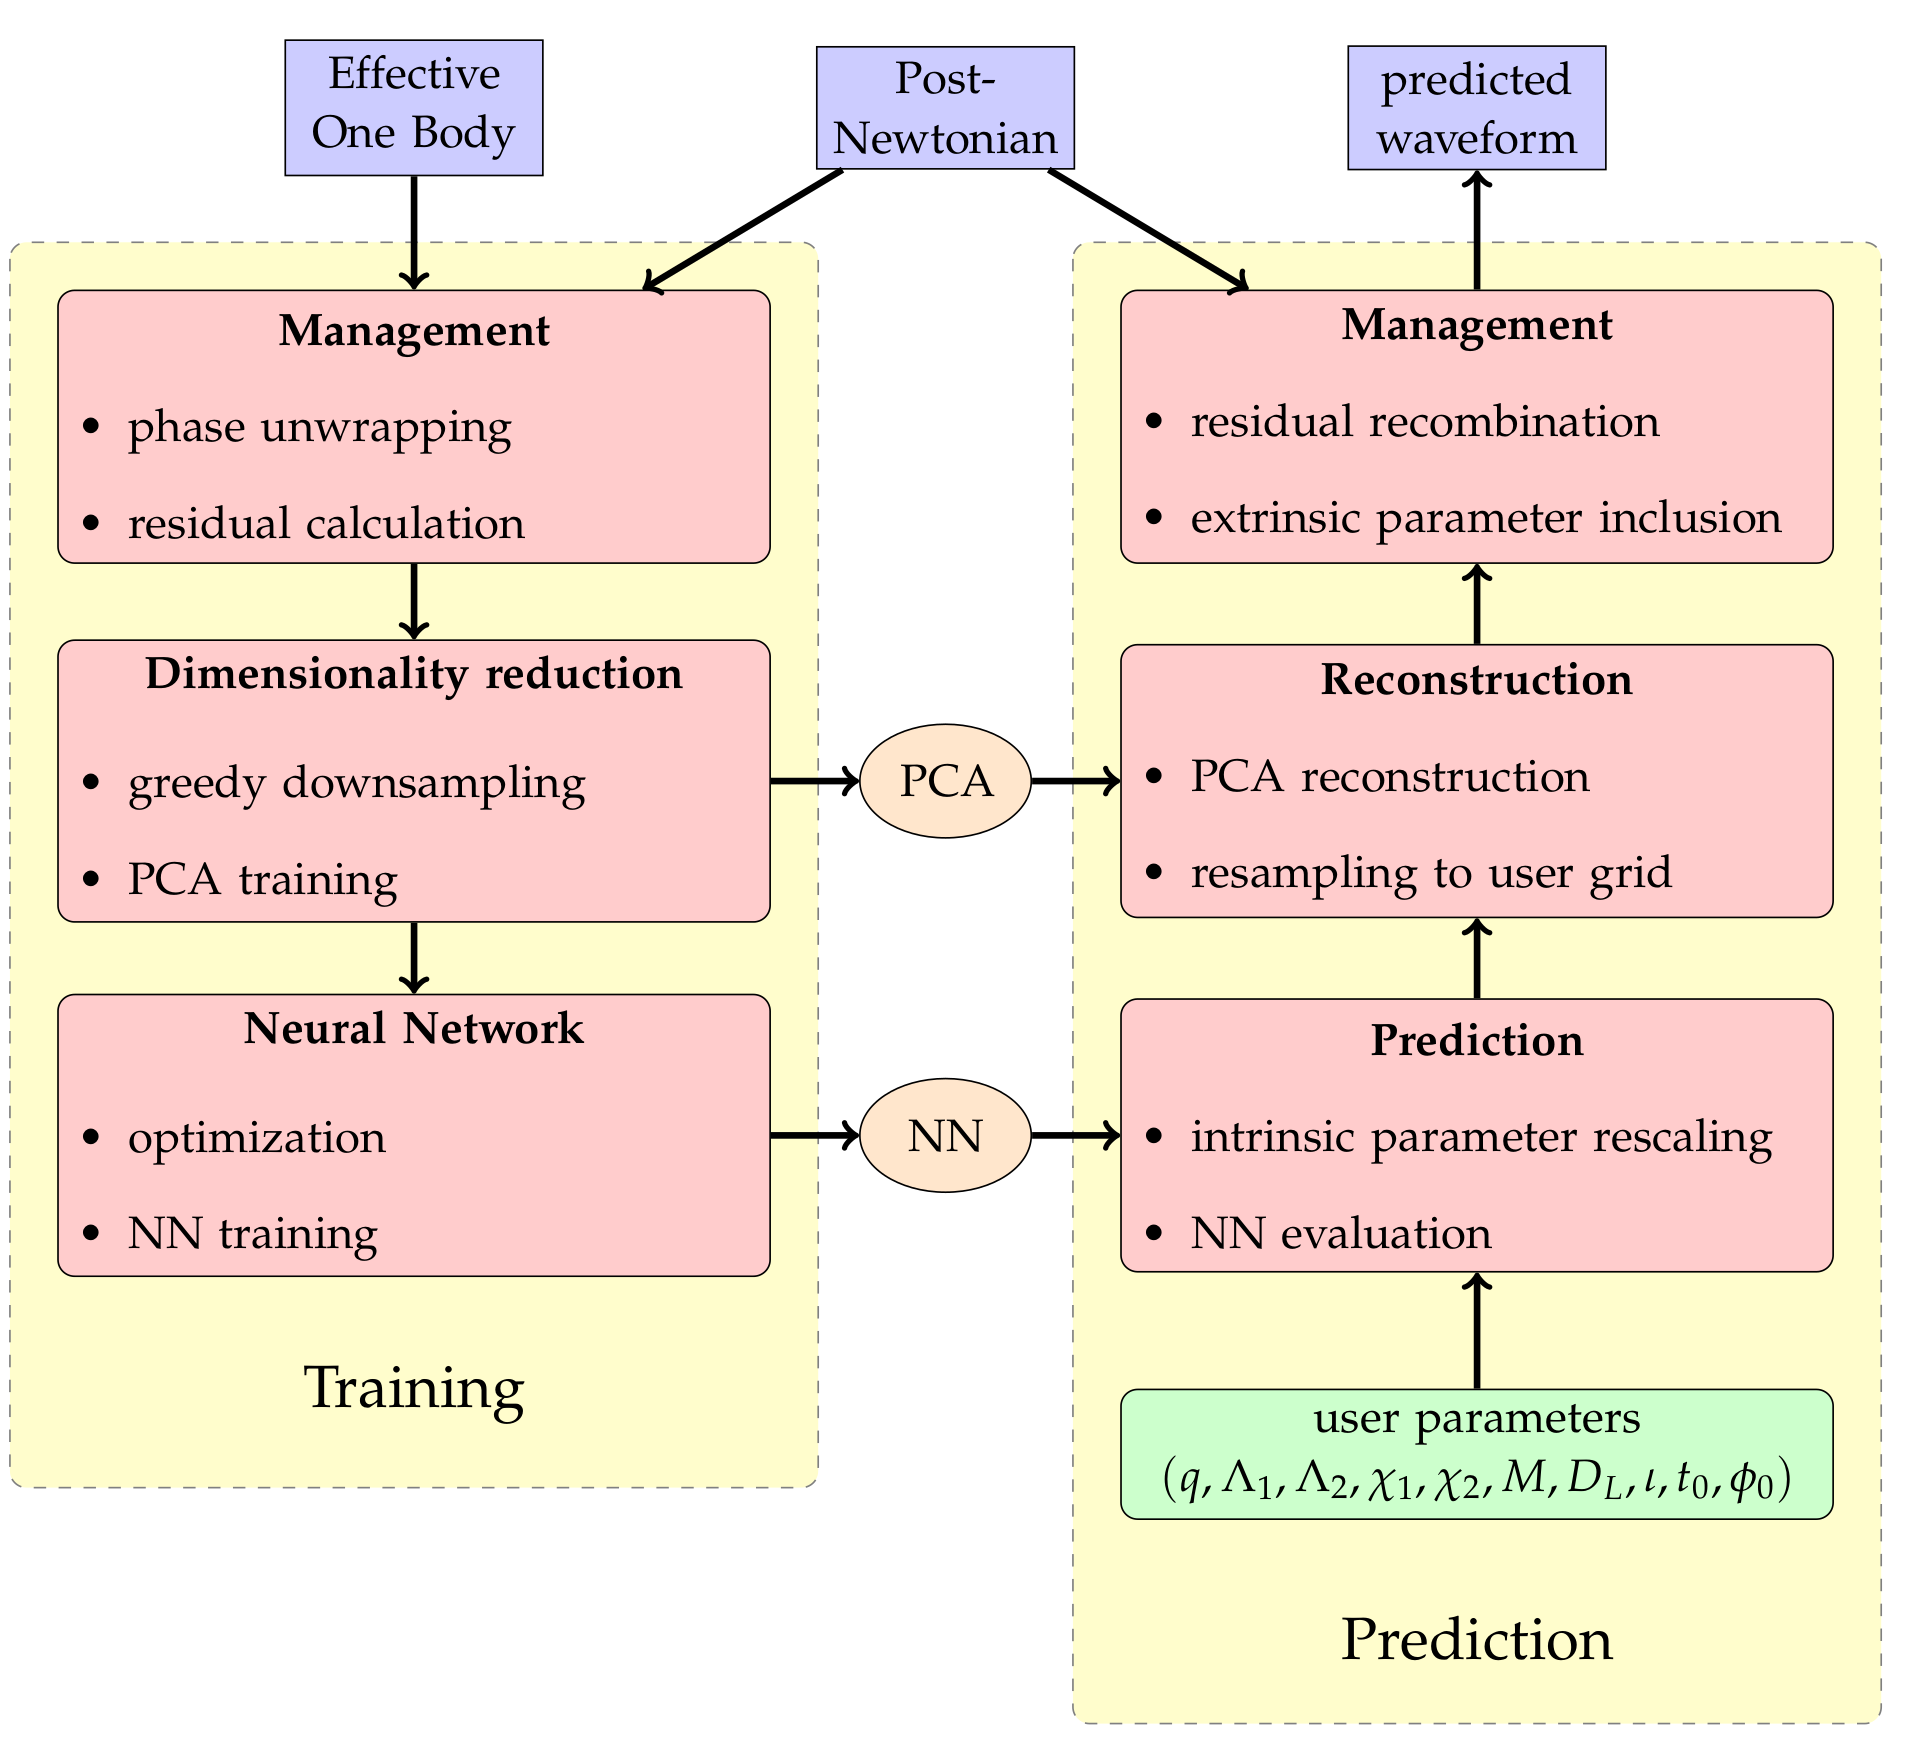
\includegraphics[width=.775\textwidth]{figures/flowchart}
    \label{fig:flowchart}
    \end{figure}
\end{frame}

\begin{frame}
    \frametitle{Residuals: amplitude}
    \begin{figure}[ht]
    \centering
    \includegraphics[width=\textwidth]{figures/amp_residuals}
    \label{fig:amp_residuals}
    \end{figure}
\end{frame}

\begin{frame}
    \frametitle{Residuals: phase}
    \begin{figure}[ht]
    \centering
    \includegraphics[width=\textwidth]{figures/phase_residuals}
    \label{fig:phase_residuals}
    \end{figure}
\end{frame}


\begin{frame}
    \frametitle{PCA mismatches}
    \begin{figure}[ht]
    \centering
    \includegraphics[width=.9\textwidth]{figures/mismatches_PCA}
    \label{fig:mismatches_PCA}
    \end{figure}
\end{frame}

\begin{frame}
    \frametitle{Hyperparameter optimization}
    \begin{figure}[ht]
    \centering
    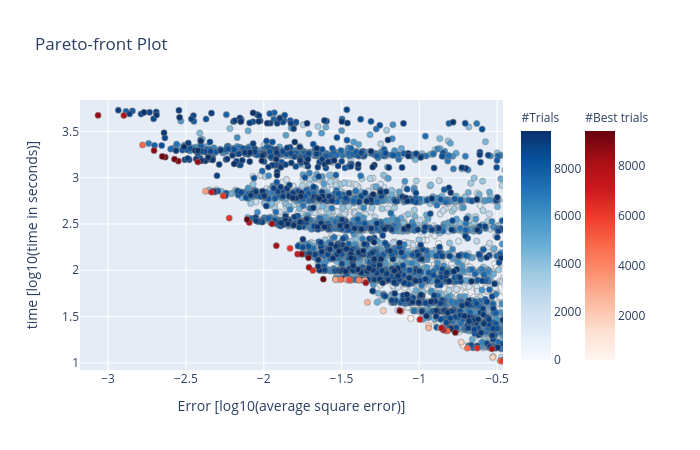
\includegraphics[width=\textwidth]{figures/pareto-front}
    \label{fig:pareto-front-nonspinning}
    \end{figure}
\end{frame}

\begin{frame}
    \frametitle{Fidelity}
    \begin{figure}[ht]
    \centering
    \includegraphics[width=\textwidth]{figures/mismatches_by_n_train_ET}
    \end{figure}
\end{frame}

\begin{frame}
    \frametitle{Amplitude reconstruction residuals}
    \begin{figure}[ht]
    \centering
    \includegraphics[width=\textwidth]{figures/recon-amp-residuals}
    \label{fig:recon-amp-residuals}
    \end{figure}
\end{frame}

\begin{frame}
    \frametitle{Phase reconstruction residuals}
    \begin{figure}[ht]
    \centering
    \includegraphics[width=\textwidth]{figures/recon-phase-residuals}
    \label{fig:recon-phase-residuals}
    \end{figure}
\end{frame}

\begin{frame}
    \frametitle{Evaluation time, varying initial frequency.}    
    \begin{figure}[ht]
    \centering
    \includegraphics[width=\textwidth]{figures/profiling_by_f0}
    \label{fig:profiling_by_f0}
    \end{figure}
\end{frame}

\begin{frame}
    \frametitle{Evaluation time, varying initial frequency.}    
    \begin{figure}[ht]
    \centering
    \includegraphics[width=\textwidth]{figures/profiling_by_f0_ratios}
    \label{fig:profiling_by_f0_ratios}
    \end{figure}
\end{frame}



\begin{frame}
    \frametitle{Evaluation time: \(f_0 = \SI{12}{Hz}\), downsampling.}    
    \begin{figure}[ht]
    \centering
    \includegraphics[width=\textwidth]{figures/profiling_by_ds}
    \label{fig:profiling_by_ds}
    \end{figure}
\end{frame}

\begin{frame}
    \frametitle{Profiling the evaluation: \(\num{2e6}\) interpolation points}
    \begin{figure}[ht]
    \centering
    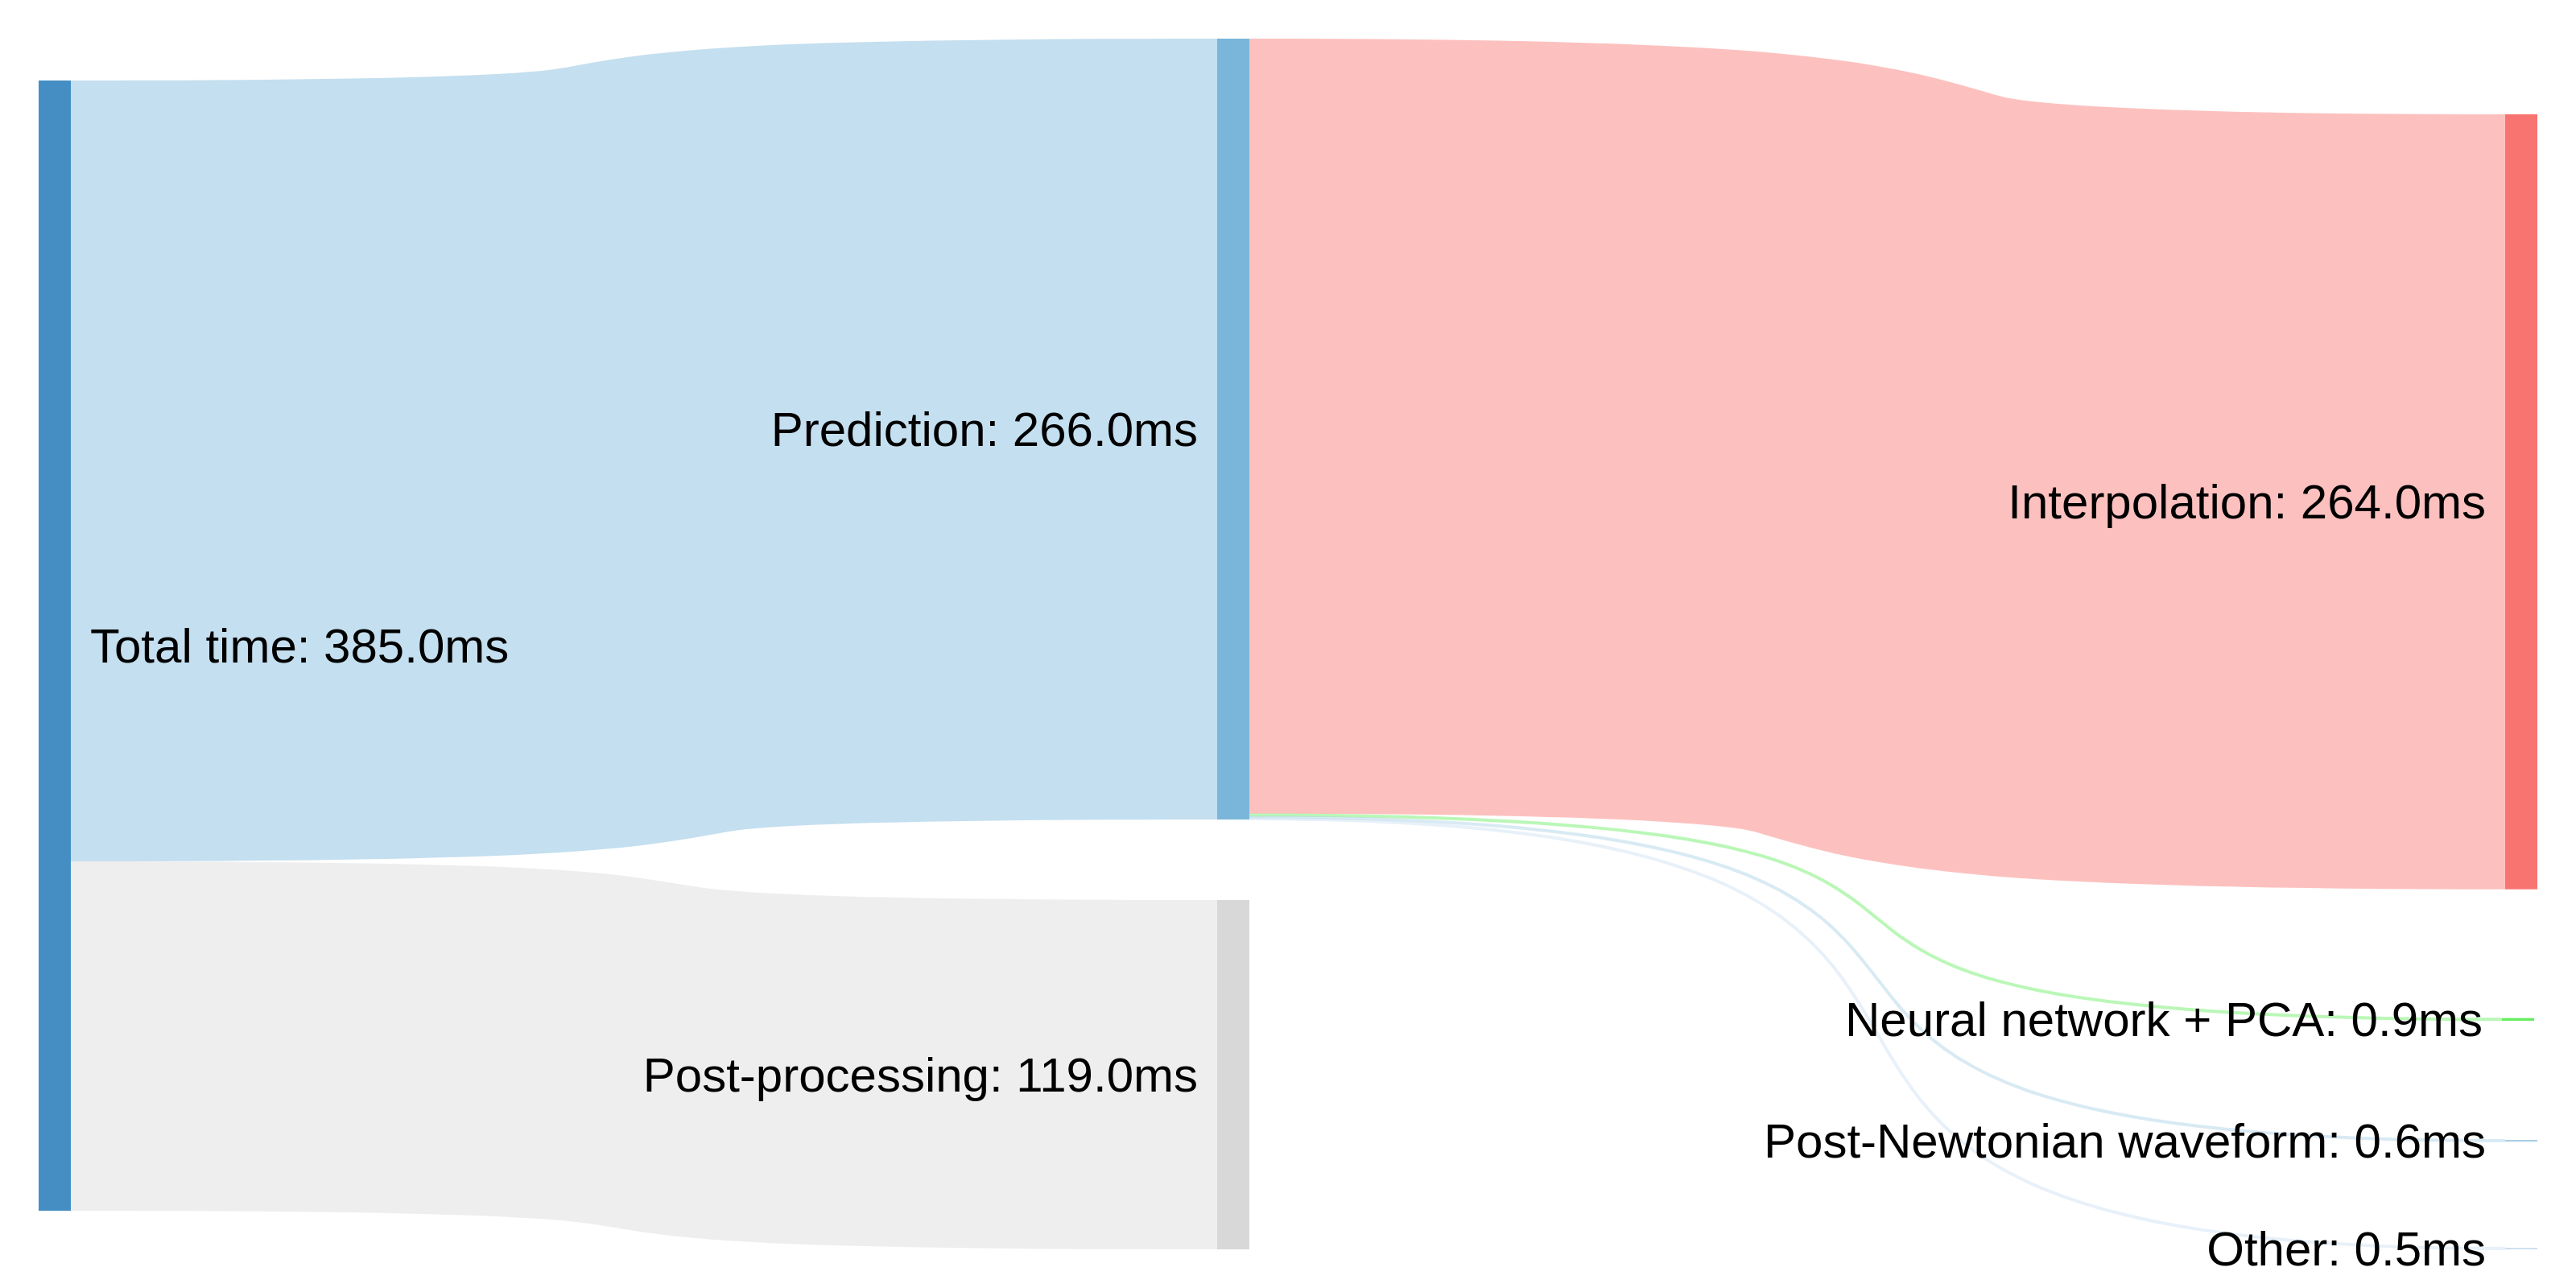
\includegraphics[width=\textwidth]{figures/sankey_full}
    \label{fig:sankey_full}
    \end{figure}
\end{frame}

\begin{frame}
    \frametitle{Profiling the evaluation: \(\num{8e3}\) interpolation points}
    \begin{figure}[ht]
    \centering
    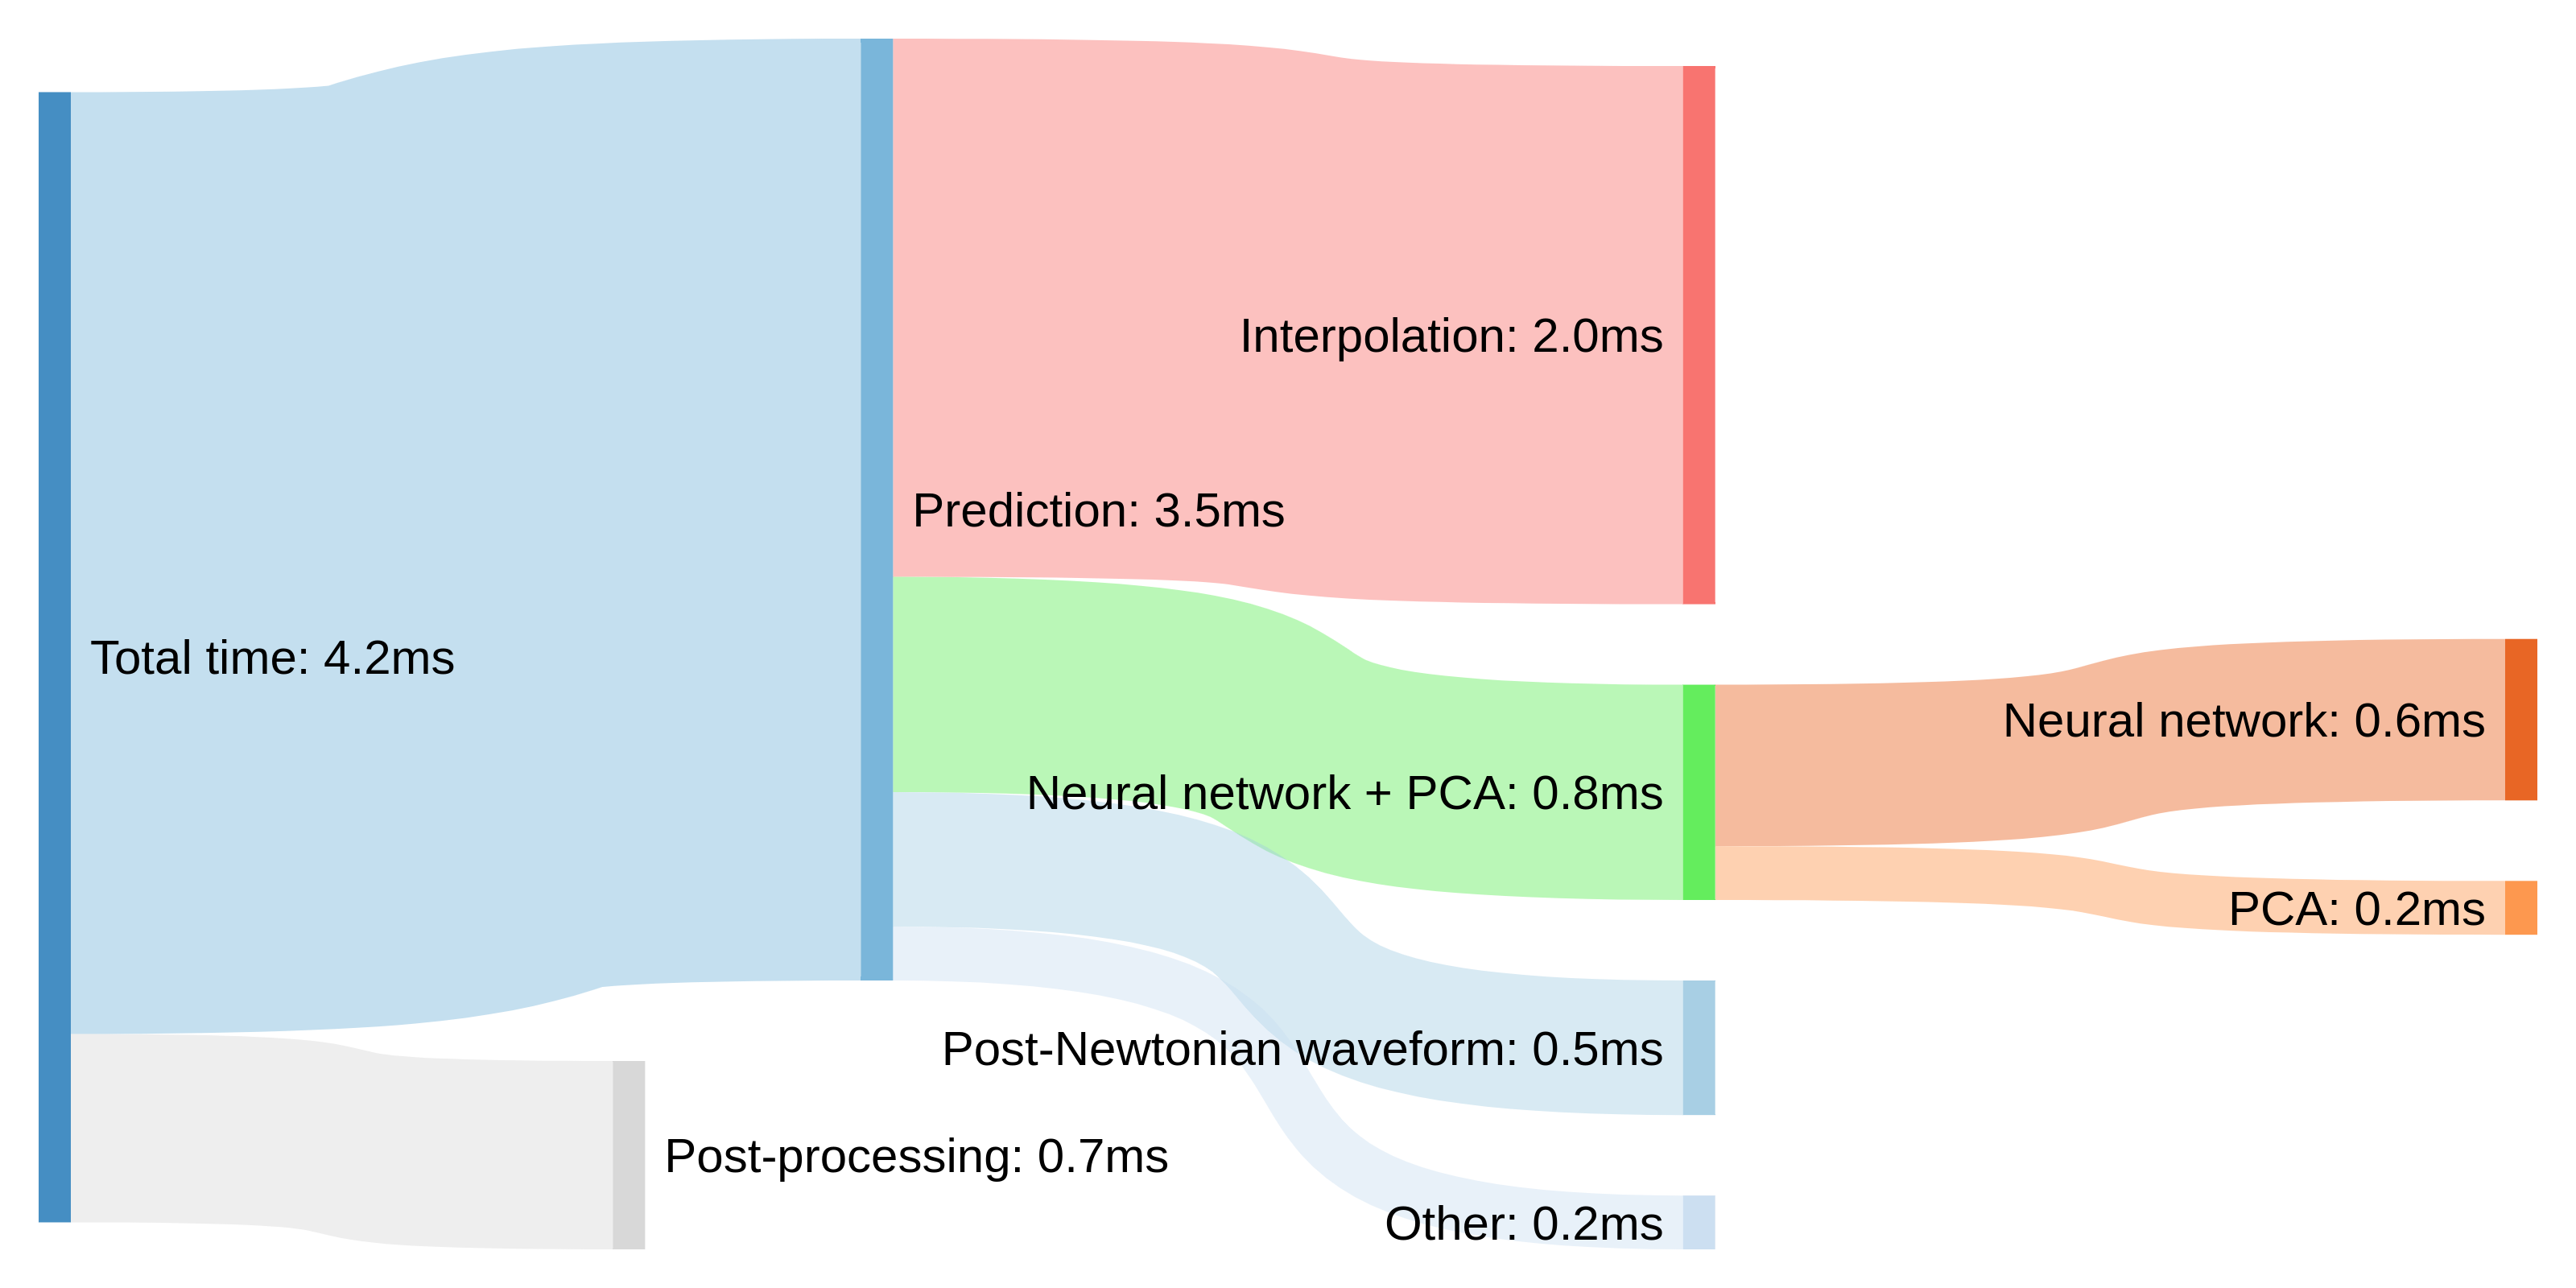
\includegraphics[width=\textwidth]{figures/sankey_downsampled}
    \label{fig:sankey_downsampled}
    \end{figure}
\end{frame}

\begin{frame}
    \frametitle{Conclusions}
    \begin{itemize}
        \item \texttt{mlgw\_bns} is a surrogate model trained on effective one body waveforms;
        \item it is accurate (enough not to bias parameter estimation);
        \item it is fast(er than the state-of-the-art model it is trained on).
    \end{itemize}
\end{frame}

\section{Backup slides}

\begin{frame}
    \frametitle{Fourier transform issues}
    
    \begin{figure}[ht]
    \centering
    \includegraphics[width=\textwidth]{figures/FFT-noise-wide}
    \label{fig:fft-noise-wide}
    \end{figure}
\end{frame}

\begin{frame}
    \frametitle{Fourier transform issues}
    \begin{figure}[ht]
    \centering
    \includegraphics[width=\textwidth]{figures/FFT-noise-highf}
    \label{fig:fft-noise-highf}
    \end{figure}
\end{frame}

\begin{frame}
    \frametitle{Fourier transform issues}
    \begin{figure}[ht]
    \centering
    \includegraphics[width=\textwidth]{figures/FFT-noise-lowf}
    \label{fig:fft-noise-lowf}
    \end{figure}
\end{frame}

\begin{frame}
    \frametitle{Natural units and quadrupolar approximation}
    \begin{align}
    \frac{\abs{\widetilde{h}(f)}}{M} &\approx \frac{1}{\pi^{2/3}} \sqrt{\frac{5}{24}} (Mf)^{-7/6} \frac{M}{r} \sqrt{\frac{m_1 m_2 }{M^2}} \\
    \abs{h_{+}(f)} &= \frac{1 + \cos^2 \iota }{2} \abs{h (f)} \\
    \abs{h_{ \times }(f)} &= \cos \iota  \abs{h (f)}
    \,.
    \end{align}
\end{frame}

\begin{frame}
    \frametitle{Fidelity requirements}
    For detection: with a mismatch \(\mathcal{F}\) we miss approximately a fraction 
    %
    \begin{align}
    1 - (1 - \mathcal{F})^3
    \end{align}
    %
    of the signals. 
    
    For parameter estimation: in order for the modelling error to be at a \(1 \sigma \) level we need 
    %
    \begin{align}
    \mathcal{F} \lesssim \frac{D}{2 \text{SNR}^2}
    \,,
    \end{align}
    %
    where \(D\) is the number of intrinsic parameters we estimate.
\end{frame}

\begin{frame}
    \frametitle{Power Spectral densities and GW170817}
    \begin{figure}[ht]
    \centering
    \vspace*{-.25cm}
    \includegraphics[width=.95\textwidth]{figures/characteristic_strains}
    \label{fig:characteristic_strains}
    \end{figure}
\end{frame}

\begin{frame}
    \frametitle{Bibliography}
    \printbibliography
\end{frame}


\end{document}
